% SPDX-License-Identifier: PMPL-1.0-or-later
% Copyright (c) 2026 Jonathan D.A. Jewell (hyperpolymath) <j.d.a.jewell@open.ac.uk>
%
% arXiv-style academic paper describing the Hypatia neurosymbolic CI/CD
% intelligence system. Intended for submission to arXiv cs.SE / cs.AI.

\documentclass[11pt,a4paper]{article}

% --- Packages ---
\usepackage[utf8]{inputenc}
\usepackage[T1]{fontenc}
\usepackage{amsmath,amssymb,amsthm}
\usepackage{graphicx}
\usepackage{booktabs}
\usepackage{hyperref}
\usepackage{algorithm}
\usepackage{algpseudocode}
\usepackage{listings}
\usepackage{xcolor}
\usepackage{tikz}
\usetikzlibrary{arrows.meta,positioning,shapes.geometric,fit,calc}
\usepackage{enumitem}
\usepackage[margin=1in]{geometry}
\usepackage{natbib}
\usepackage{subcaption}
\usepackage{multirow}

% --- Theorem environments ---
\newtheorem{definition}{Definition}
\newtheorem{theorem}{Theorem}
\newtheorem{proposition}{Proposition}

% --- Listings style ---
\lstset{
  basicstyle=\ttfamily\small,
  keywordstyle=\color{blue!70!black}\bfseries,
  commentstyle=\color{green!50!black}\itshape,
  stringstyle=\color{red!60!black},
  breaklines=true,
  frame=single,
  numbers=left,
  numberstyle=\tiny\color{gray},
  captionpos=b
}

% --- Title ---
\title{%
  \textbf{From Detection to Decision: Neurosymbolic Intelligence\\
  for CI/CD Remediation Orchestration}
}

\author{
  Jonathan D.A. Jewell\\
  \texttt{j.d.a.jewell@open.ac.uk}\\
  \textit{Independent Researcher}
}

\date{March 2026}

\begin{document}

\maketitle

% ============================================================
% ABSTRACT
% ============================================================
\begin{abstract}
Modern software supply chains deploy numerous static and dynamic analysis tools---CodeQL, Semgrep, Snyk, Trivy, SonarQube---that collectively generate thousands of findings per organisation. Yet the critical gap is not \emph{detection} but \emph{decision}: given a finding, what should be done, by whom, with what confidence, and in what order? We present \textsc{Hypatia}, a neurosymbolic decision intelligence system that sits between scanners and fixers in CI/CD pipelines, orchestrating automated remediation across a fleet of specialised bots. \textsc{Hypatia} combines five lightweight neural networks---a trust-weighted PageRank graph, a sparse Mixture of Experts, two reservoir computing networks (Liquid State Machine and Echo State Network), and a Radial Basis Function novelty detector---with 20 declarative Logtalk/Prolog rules for known standards compliance. A Safety Triangle framework inspired by occupational hazard hierarchies routes every finding through Eliminate, Substitute, or Control tiers with confidence-gated dispatch. Over 16{,}671 recorded outcomes across 302 repositories, the system achieves a 99\% remediation success rate with Bayesian confidence updating, automatic bot quarantine on failure streaks, and batch rollback capability. We argue that this detection--decision decoupling represents a necessary paradigm shift for managing the combinatorial explosion of findings in modern DevSecOps environments.

\medskip
\noindent\textbf{Keywords:} neurosymbolic AI, CI/CD, automated remediation, software engineering intelligence, safety triangle, DevSecOps, reservoir computing
\end{abstract}

% ============================================================
% 1. INTRODUCTION
% ============================================================
\section{Introduction}
\label{sec:introduction}

The modern software development organisation faces a paradox of abundance. A single repository integrated with GitHub Advanced Security, Snyk, SonarQube, and an OpenSSF Scorecard check may surface hundreds of findings per commit. Across an ecosystem of hundreds of repositories, the aggregate volume easily reaches thousands of actionable---and many non-actionable---alerts. The tools responsible for this output are increasingly sophisticated: CodeQL performs deep dataflow analysis \citep{codeql2019}, Semgrep enables pattern-based detection at scale \citep{semgrep2020}, and Trivy scans container images against comprehensive vulnerability databases \citep{trivy2019}. Detection, in short, is a solved problem at the individual-finding level.

What remains unsolved is the \emph{decision} problem. For each finding, an engineer must determine:
\begin{enumerate}[nosep]
  \item Is this a true positive or a false positive?
  \item If true, what is the correct remediation?
  \item Can the remediation be automated, or does it require human judgement?
  \item What is the confidence that the automated fix will succeed?
  \item In what order should remediations be applied to avoid conflicts?
  \item How should we update our confidence in the remediation recipe based on outcomes?
\end{enumerate}

\noindent These questions are fundamentally different from detection questions. They require contextual reasoning about trust, temporal patterns, domain expertise, and organisational policy---precisely the kind of reasoning that falls between the cracks of existing tooling.

Dependabot \citep{dependabot2017} and Renovate \citep{renovate2017} automate dependency updates but operate in isolation from security findings. CodeQL autofixes \citep{codeql-autofix2024} generate patches but lack confidence estimation or fleet coordination. The result is a fragmented landscape where each tool makes local decisions without global context.

This paper presents \textsc{Hypatia}\footnote{Named after Hypatia of Alexandria (c.\ 350--415 CE), mathematician, astronomer, and philosopher---one of the last scholars of the Library of Alexandria.}, a neurosymbolic decision intelligence system designed to occupy the architectural gap between scanners and fixers. \textsc{Hypatia} does not scan code. It does not generate patches. Instead, it receives findings from upstream scanners, applies a combination of neural and symbolic reasoning to estimate confidence and select remediation strategies, routes actions through a Safety Triangle hierarchy, and dispatches work to a fleet of specialised bots---tracking outcomes to continuously update its models.

The contributions of this paper are:
\begin{enumerate}[nosep]
  \item A formal articulation of the \emph{detection--decision gap} in CI/CD pipelines and the argument that it constitutes a distinct architectural concern (Section~\ref{sec:paradigm}).
  \item A neurosymbolic architecture combining five specialised neural networks with declarative symbolic rules, with clear criteria for when neural versus symbolic reasoning is appropriate (Section~\ref{sec:architecture}).
  \item A Safety Triangle remediation routing framework adapted from occupational safety hierarchies (Section~\ref{sec:triangle}).
  \item A multi-tier bot orchestration system with confidence-gated dispatch, automatic quarantine, and batch rollback (Section~\ref{sec:fleet}).
  \item Empirical results from deployment across 302 repositories with 16{,}671 recorded outcomes (Section~\ref{sec:evaluation}).
\end{enumerate}


% ============================================================
% 2. BACKGROUND
% ============================================================
\section{Background and Related Concepts}
\label{sec:background}

\subsection{Static and Dynamic Analysis in CI/CD}

The maturation of CI/CD practices has driven widespread adoption of automated analysis tools. Static Application Security Testing (SAST) tools such as CodeQL \citep{codeql2019}, Semgrep \citep{semgrep2020}, and SonarQube \citep{sonarqube2006} analyse source code without execution, identifying potential vulnerabilities, code smells, and compliance violations. Dynamic Application Security Testing (DAST) tools like OWASP ZAP probe running applications. Software Composition Analysis (SCA) tools including Snyk \citep{snyk2015}, Trivy \citep{trivy2019}, and Grype analyse dependency manifests against vulnerability databases.

These tools are complementary in coverage but produce findings in heterogeneous formats---SARIF, JSON, proprietary dashboards---with no unified model for priority, confidence, or remediation strategy. The SARIF standard \citep{sarif2018} provides a common interchange format for findings but deliberately excludes remediation semantics.

\subsection{Automated Remediation}

Existing automated remediation falls into three categories:

\begin{description}[nosep]
  \item[Dependency updaters:] Dependabot \citep{dependabot2017}, Renovate \citep{renovate2017}, and Mend update dependency versions automatically. These are effective for known CVEs with patch versions available but cannot address code-level vulnerabilities.
  \item[Autofix engines:] CodeQL autofix \citep{codeql-autofix2024} and Semgrep autofix generate source patches for detected patterns. These operate per-finding without cross-finding coordination or confidence tracking.
  \item[Security orchestrators:] Platforms like Snyk and Mend offer centralised dashboards but focus on prioritisation (which findings matter) rather than orchestrated execution (what to do about them).
\end{description}

\noindent None of these systems maintain a feedback loop from remediation outcomes back to confidence estimation. None coordinate across a fleet of specialised agents. None distinguish between findings that can be eliminated automatically, those requiring substitution with verified alternatives, and those requiring human control.

\subsection{Neural Networks for Software Engineering}

The application of neural networks to software engineering has expanded rapidly. Code completion models (Codex, CodeLlama) generate code from natural language. Defect prediction models estimate bug probability from code features \citep{wang2016}. Vulnerability detection models learn patterns of insecure code \citep{li2018}.

However, the application of neural networks to \emph{remediation orchestration}---deciding what to do about known findings---remains underexplored. This is the space \textsc{Hypatia} occupies: not detecting vulnerabilities, but making operational decisions about detected vulnerabilities.

\subsection{Neurosymbolic AI}

Neurosymbolic AI combines neural learning with symbolic reasoning to exploit the strengths of both paradigms \citep{garcez2019}. Neural components handle pattern recognition, uncertainty quantification, and generalisation from data. Symbolic components enforce hard constraints, encode domain knowledge, and provide interpretable decisions.

In \textsc{Hypatia}, the neurosymbolic split follows a clear principle: \emph{use symbolic rules for known-knowns; use neural networks for known-unknowns and unknown-unknowns}. The 20 OpenSSF Scorecard compliance checks, for instance, have deterministic correct answers---symbolic rules handle these without wasting neural capacity. Whether a novel finding category requires security expertise or documentation expertise---that is a learned judgement for the Mixture of Experts.


% ============================================================
% 3. FROM DETECTION TO DECISION
% ============================================================
\section{From Detection to Decision: The Paradigm Shift}
\label{sec:paradigm}

\subsection{The Detection--Decision Gap}

We define the \emph{detection--decision gap} as the architectural void between tools that identify problems and systems that resolve them. Formally:

\begin{definition}[Detection--Decision Gap]
Given a set of scanners $S = \{s_1, \ldots, s_n\}$ each producing findings $F_i = s_i(R)$ for repository $R$, the detection--decision gap is the set of decisions $D = \{d_1, \ldots, d_m\}$ required to transform $\bigcup F_i$ into a sequence of remediation actions $A = \langle a_1, \ldots, a_k \rangle$ that respects ordering constraints, confidence thresholds, and organisational policy.
\end{definition}

The gap is not merely a missing feature---it is a missing \emph{architectural layer}. Scanners are designed to be conservative (minimise false negatives), which necessarily produces false positives. Fixers are designed to be precise (apply exact patches), which necessarily requires confident input. Between conservatism and precision lies a judgement layer that current toolchains lack.

\subsection{Why the Gap Persists}

Three structural factors perpetuate the detection--decision gap:

\textbf{Tool silos.} Each scanner operates independently with its own severity model, false positive rate, and output format. A CodeQL \texttt{HIGH} is not commensurable with a Trivy \texttt{CRITICAL} without contextual normalisation.

\textbf{Absence of feedback loops.} When Dependabot creates a pull request, no system records whether the PR was merged, reverted, or ignored---and feeds that outcome back to adjust future confidence. Each remediation attempt is statistically independent.

\textbf{The coordination problem.} Fixing finding $f_1$ may invalidate finding $f_2$ (e.g., updating a dependency resolves both a CVE and a license violation). Without cross-finding awareness, tools generate conflicting or redundant remediations.

\subsection{Decision Intelligence as a First-Class Concern}

\textsc{Hypatia}'s core architectural claim is that \emph{remediation decision-making deserves its own system}, distinct from both scanners and fixers. This system must:

\begin{enumerate}[nosep]
  \item Ingest findings from heterogeneous scanners into a normalised model.
  \item Estimate confidence in candidate remediations using both learned patterns and domain rules.
  \item Route findings through a hazard hierarchy that distinguishes automation-safe from human-required decisions.
  \item Dispatch actions to specialised execution agents with appropriate gating.
  \item Record outcomes and update models continuously.
\end{enumerate}

\noindent This is the architecture \textsc{Hypatia} implements, described in the following sections.


% ============================================================
% 4. THE NEUROSYMBOLIC ARCHITECTURE
% ============================================================
\section{The Neurosymbolic Architecture}
\label{sec:architecture}

\textsc{Hypatia}'s architecture comprises a neural layer of five specialised networks, a symbolic layer of 20 declarative rules, a coordination layer that fuses their outputs, and a safety/dispatch layer that translates decisions into actions. Figure~\ref{fig:architecture} illustrates the overall pipeline.

\begin{figure}[htbp]
\centering
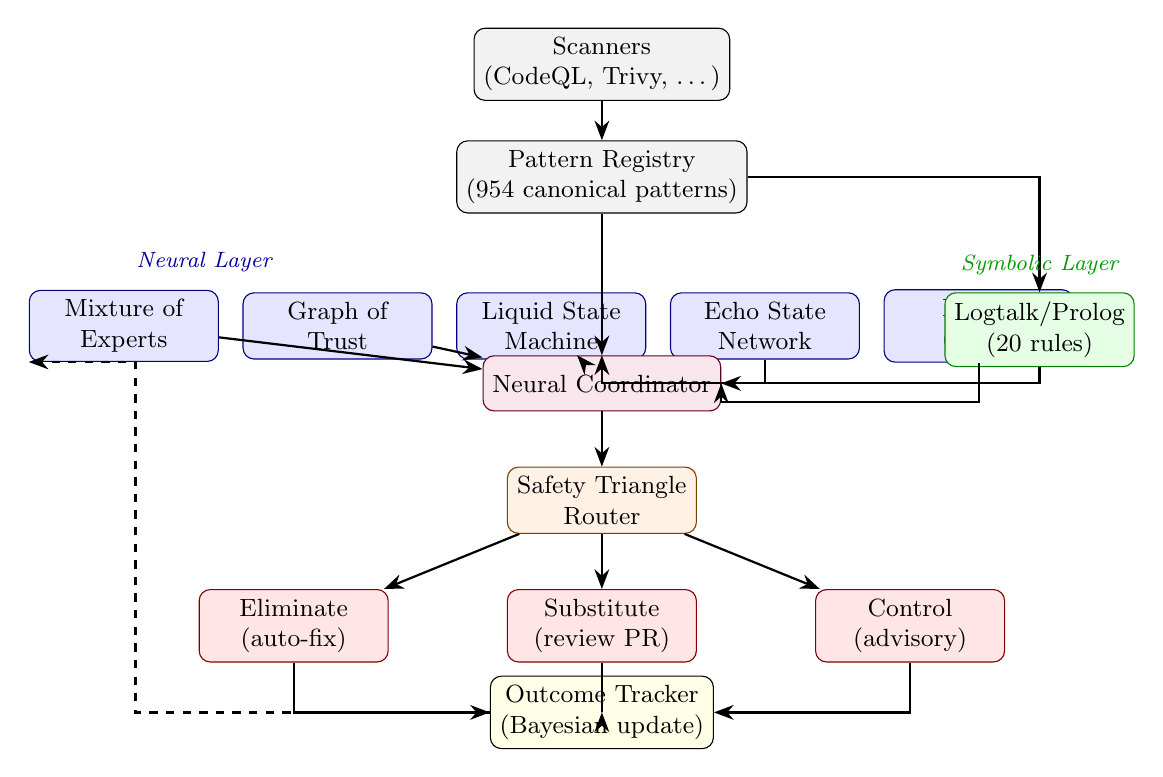
\begin{tikzpicture}[
  node distance=0.7cm and 1.2cm,
  box/.style={rectangle, draw, rounded corners, minimum width=2.4cm, minimum height=0.7cm, align=center, font=\small},
  neuralbox/.style={box, fill=blue!10, draw=blue!50!black},
  symbox/.style={box, fill=green!10, draw=green!50!black},
  safetybox/.style={box, fill=orange!10, draw=orange!50!black},
  dispatchbox/.style={box, fill=red!10, draw=red!50!black},
  arr/.style={-{Stealth[length=2.5mm]}, thick},
  darr/.style={-{Stealth[length=2.5mm]}, thick, dashed}
]

% Input
\node[box, fill=gray!10] (scanners) {Scanners\\(CodeQL, Trivy, \ldots)};
\node[box, fill=gray!10, below=0.5cm of scanners] (registry) {Pattern Registry\\(954 canonical patterns)};

% Neural layer
\node[neuralbox, below left=1.0cm and 0.3cm of registry] (got) {Graph of\\Trust};
\node[neuralbox, left=0.3cm of got] (moe) {Mixture of\\Experts};
\node[neuralbox, right=0.3cm of got] (lsm) {Liquid State\\Machine};
\node[neuralbox, right=0.3cm of lsm] (esn) {Echo State\\Network};
\node[neuralbox, right=0.3cm of esn] (rbf) {Radial\\(RBF)};

% Symbolic layer
\node[symbox, below right=1.0cm and 2.5cm of registry] (rules) {Logtalk/Prolog\\(20 rules)};

% Coordinator
\node[box, fill=purple!10, draw=purple!50!black, below=1.8cm of registry] (coord) {Neural Coordinator};

% Triangle
\node[safetybox, below=0.7cm of coord] (triangle) {Safety Triangle\\Router};

% Dispatch tiers
\node[dispatchbox, below left=0.7cm and 1.5cm of triangle] (elim) {Eliminate\\(auto-fix)};
\node[dispatchbox, below=0.7cm of triangle] (sub) {Substitute\\(review PR)};
\node[dispatchbox, below right=0.7cm and 1.5cm of triangle] (ctrl) {Control\\(advisory)};

% Outcome
\node[box, fill=yellow!10, below=1.8cm of triangle] (outcome) {Outcome Tracker\\(Bayesian update)};

% Arrows
\draw[arr] (scanners) -- (registry);
\draw[arr] (registry) -- (coord);
\draw[arr] (registry) -| (rules);
\draw[arr] (moe) -- (coord);
\draw[arr] (got) -- (coord);
\draw[arr] (lsm) -- (coord);
\draw[arr] (esn.south) -- ++(0,-0.3) -| (coord);
\draw[arr] (rbf.south) -- ++(0,-0.5) -| (coord.east);
\draw[arr] (rules) |- (coord);
\draw[arr] (coord) -- (triangle);
\draw[arr] (triangle) -- (elim);
\draw[arr] (triangle) -- (sub);
\draw[arr] (triangle) -- (ctrl);
\draw[arr] (elim) |- (outcome);
\draw[arr] (sub) |- (outcome);
\draw[arr] (ctrl) |- (outcome);
\draw[darr] (outcome.west) -- ++(-4.5,0) |- (moe.south west);

% Labels
\node[above=0.1cm of moe, font=\footnotesize\itshape, blue!60!black, anchor=south east, xshift=2cm] {Neural Layer};
\node[above=0.1cm of rules, font=\footnotesize\itshape, green!60!black] {Symbolic Layer};

\end{tikzpicture}
\caption{The \textsc{Hypatia} neurosymbolic pipeline. Findings flow from scanners through the pattern registry, are evaluated by five neural networks and 20 symbolic rules, fused by the coordinator, routed through the Safety Triangle, dispatched to execution bots, and outcomes feed back to update models.}
\label{fig:architecture}
\end{figure}


\subsection{The Neural Layer: Five Specialised Networks}
\label{subsec:neural}

Each neural network in \textsc{Hypatia} serves a distinct cognitive function in the decision pipeline. The design philosophy is \emph{many small specialists} rather than one large generalist: each network is lightweight (hundreds of parameters, not millions), interpretable, and independently trainable from operational data.

\subsubsection{Graph of Trust (PageRank)}
\label{subsubsec:got}

The Graph of Trust models trust relationships between repositories, bots, and remediation recipes as a directed citation graph. When bot $b$ successfully applies recipe $r$ to repository $\rho$, a directed edge $(\rho, r, b)$ is created with weight proportional to the outcome's confidence delta.

Trust propagation follows a modified PageRank formulation:

\begin{equation}
\text{Trust}(v) = \frac{1 - d}{N} + d \sum_{u \in \text{in}(v)} \frac{\text{Trust}(u) \cdot w(u, v)}{\sum_{z \in \text{out}(u)} w(u, z)}
\label{eq:trust}
\end{equation}

\noindent where $d = 0.85$ is the damping factor and $w(u, v)$ is the outcome-weighted edge strength. This enables transitive trust: if recipe $r_1$ is trusted for repositories similar to $\rho_2$, the trust propagates---but attenuates with distance.

The trust graph serves two operational functions: (a) selecting which bot should handle a finding, based on the bot's trust score for that finding category, and (b) estimating recipe confidence for repositories not yet encountered, by propagating trust from similar repositories.

\subsubsection{Mixture of Experts (Sparse MoE)}
\label{subsubsec:moe}

The Mixture of Experts network routes each finding to domain-specific expert sub-networks for confidence estimation. Seven expert domains are defined:

\begin{enumerate}[nosep]
  \item \textbf{Security}: CVEs, vulnerabilities, secret exposure, injection flaws.
  \item \textbf{Quality}: Code complexity, duplication, dead code, style violations.
  \item \textbf{Sustainability}: License compliance, dependency health, SBOM coverage.
  \item \textbf{Accessibility}: WCAG compliance, a11y issues in web frontends.
  \item \textbf{Performance}: Resource leaks, algorithmic complexity, caching misses.
  \item \textbf{Documentation}: Missing or outdated documentation, API coverage.
  \item \textbf{Infrastructure}: CI/CD configuration, container security, deployment hygiene.
\end{enumerate}

The gating network computes a softmax distribution over experts given an input feature vector $\mathbf{x}$:

\begin{equation}
g_i(\mathbf{x}) = \frac{\exp(\mathbf{w}_i^\top \mathbf{x})}{\sum_{j=1}^{7} \exp(\mathbf{w}_j^\top \mathbf{x})}
\label{eq:gating}
\end{equation}

For efficiency, only the top-$k$ experts (with $k=2$) are activated per finding, following the sparse MoE paradigm of \citet{shazeer2017}. An auxiliary load-balancing loss prevents expert collapse:

\begin{equation}
\mathcal{L}_{\text{balance}} = \lambda \sum_{i=1}^{7} \left( f_i - \frac{1}{7} \right)^2
\label{eq:balance}
\end{equation}

\noindent where $f_i$ is the fraction of findings routed to expert $i$ and $\lambda = 0.01$.

Each activated expert produces a confidence estimate for the finding. The final confidence is the gating-weighted combination:

\begin{equation}
c(\mathbf{x}) = \sum_{i \in \text{top-}k} g_i(\mathbf{x}) \cdot e_i(\mathbf{x})
\label{eq:moe_confidence}
\end{equation}

\subsubsection{Liquid State Machine (Reservoir Computing)}
\label{subsubsec:lsm}

The Liquid State Machine (LSM) \citep{maass2002} processes the temporal stream of findings as they arrive, maintaining a dynamic reservoir state that captures short-term and medium-term patterns. Its primary function is \emph{temporal anomaly detection}: identifying sudden changes in finding volume, category distribution, or severity that may signal deployment incidents or scanner misconfiguration.

The reservoir state evolves as:

\begin{equation}
\mathbf{h}(t) = f\!\left( \mathbf{W}_{\text{in}} \mathbf{x}(t) + \mathbf{W}_{\text{res}} \mathbf{h}(t-1) \right)
\label{eq:lsm}
\end{equation}

\noindent where $\mathbf{W}_{\text{in}}$ is the input weight matrix, $\mathbf{W}_{\text{res}}$ is the sparse recurrent reservoir matrix (spectral radius $< 1$ for echo state property), and $f$ is a nonlinear activation. The reservoir is not trained; only a linear readout layer $\mathbf{W}_{\text{out}}$ is trained to predict the expected finding rate, with deviations flagged as anomalies.

Operationally, the LSM triggers alerts when:
\begin{itemize}[nosep]
  \item Finding volume for a repository exceeds $2\sigma$ of its rolling average.
  \item A category that was previously absent suddenly appears (e.g., a repository with no security findings starts producing them).
  \item The temporal spacing between findings from the same scanner decreases sharply (suggesting a scanner-side issue rather than genuine new vulnerabilities).
\end{itemize}

\subsubsection{Echo State Network (Reservoir Computing)}
\label{subsubsec:esn}

The Echo State Network (ESN) \citep{jaeger2001} is structurally similar to the LSM but trained on a different signal: \emph{confidence trajectories} over time. For each recipe, the ESN tracks the sequence of confidence values after each outcome is recorded, forecasting where the confidence trajectory is heading.

The ESN detects three critical conditions:
\begin{enumerate}[nosep]
  \item \textbf{Confidence drift}: A recipe whose confidence is monotonically declining over its last $n$ applications, suggesting the recipe is becoming stale or the codebase is evolving away from it.
  \item \textbf{Oscillation}: A recipe alternating between success and failure, suggesting an intermittent environmental factor.
  \item \textbf{Plateau at sub-threshold}: A recipe whose confidence has stabilised below the auto-execute threshold (0.95), suggesting it needs human review to break through.
\end{enumerate}

Training uses the Bayesian confidence time series from the Outcome Tracker (Section~\ref{subsec:outcome}), fitting the readout weights via ridge regression:

\begin{equation}
\mathbf{W}_{\text{out}} = \mathbf{Y} \mathbf{H}^\top (\mathbf{H} \mathbf{H}^\top + \alpha \mathbf{I})^{-1}
\label{eq:esn_train}
\end{equation}

\noindent where $\mathbf{H}$ is the matrix of reservoir states and $\alpha$ is the regularisation parameter.

\subsubsection{Radial Basis Function Network (Novelty Detection)}
\label{subsubsec:rbf}

The Radial Basis Function (RBF) network serves as \textsc{Hypatia}'s novelty detector, answering the question: \emph{has this type of finding been seen before?} Each finding is represented as an 8-dimensional feature vector encoding category, severity, scanner source, language, file path pattern, dependency depth, age-since-introduction, and cross-reference count.

The RBF network computes:

\begin{equation}
\phi_i(\mathbf{x}) = \exp\!\left( -\frac{\|\mathbf{x} - \mathbf{c}_i\|^2}{2\sigma_i^2} \right)
\label{eq:rbf}
\end{equation}

\noindent where $\mathbf{c}_i$ are learned centres corresponding to known finding clusters. The output is:

\begin{equation}
y(\mathbf{x}) = \sum_{i=1}^{M} w_i \phi_i(\mathbf{x})
\label{eq:rbf_output}
\end{equation}

When $\max_i \phi_i(\mathbf{x}) < \tau_{\text{novelty}}$ (no known centre is close to the input), the finding is classified as \emph{novel} and automatically routed to the Control tier (human review required), regardless of any other confidence signal. This is a critical safety property: \textsc{Hypatia} never auto-fixes a type of finding it has not successfully remediated before.

\subsection{The Symbolic Layer: Declarative Rules}
\label{subsec:symbolic}

Twenty Logtalk/Prolog rules encode deterministic domain knowledge---the ``known-knowns'' that do not benefit from neural approximation. These rules cover:

\begin{table}[htbp]
\centering
\caption{Symbolic rule categories in \textsc{Hypatia}. Each rule is a Logtalk clause with deterministic output, avoiding neural computation overhead for well-understood checks.}
\label{tab:rules}
\begin{tabular}{@{}llc@{}}
\toprule
\textbf{Category} & \textbf{Representative Rules} & \textbf{Count} \\
\midrule
OpenSSF Scorecard & Branch protection, signed releases, SAST enabled & 6 \\
CI/CD Compliance & SHA-pinned actions, permissions declared, SPDX headers & 4 \\
Structural Drift & Banned languages detected, required files missing & 3 \\
Security Errors & MD5/SHA1 usage, HTTP URLs, hardcoded secrets & 3 \\
Code Safety & \texttt{unsafe} blocks without justification, \texttt{eval()} usage & 2 \\
Migration & Deprecated API usage, end-of-life runtime versions & 2 \\
\midrule
\textbf{Total} & & \textbf{20} \\
\bottomrule
\end{tabular}
\end{table}

The symbolic layer processes findings \emph{before} the neural layer. Any finding that matches a symbolic rule receives a deterministic verdict---either a confirmed true positive with a known recipe, or a confirmed false positive to be suppressed. Only findings not resolved by the symbolic layer proceed to neural evaluation.

This architecture has two advantages. First, it is fast: Logtalk rule evaluation is sub-millisecond, avoiding the overhead of neural inference for standard checks. Second, it is auditable: every symbolic decision can be traced to a specific rule with a human-readable justification, satisfying compliance requirements that opaque neural decisions cannot.

\subsection{Neurosymbolic Fusion}
\label{subsec:fusion}

The Neural Coordinator (implemented as an OTP GenServer in Elixir) fuses outputs from all five networks and the symbolic layer into a unified decision:

\begin{algorithm}[htbp]
\caption{Neurosymbolic Decision Fusion}
\label{alg:fusion}
\begin{algorithmic}[1]
\Require Finding $f$, repository $\rho$, language $\ell$
\Ensure Decision $d \in \{\text{eliminate}, \text{substitute}, \text{control}\}$, confidence $c$
\State \textbf{Symbolic pass:} $r_s \gets \text{SymbolicRules}(f)$
\If{$r_s$ is deterministic} \Return $r_s$ \EndIf
\State \textbf{Novelty check:} $n \gets \text{RBF}.\text{novelty}(f)$
\If{$n > \tau_{\text{novelty}}$} \Return $(\text{control}, 0.0)$ \Comment{Force human review} \EndIf
\State \textbf{Domain routing:} $c_{\text{moe}} \gets \text{MoE}.\text{confidence}(f)$
\State \textbf{Trust weighting:} $t \gets \text{GoT}.\text{trust}(\rho, f.\text{category})$
\State \textbf{Anomaly check:} $a \gets \text{LSM}.\text{anomaly}(f, \rho)$
\If{$a$ is anomalous} $c_{\text{moe}} \gets c_{\text{moe}} \times 0.5$ \Comment{Halve confidence during anomalies} \EndIf
\State \textbf{Trajectory check:} $\delta \gets \text{ESN}.\text{trend}(f.\text{recipe})$
\If{$\delta < -0.1$} flag recipe for review \EndIf
\State $c \gets c_{\text{moe}} \times t$ \Comment{Trust-weighted confidence}
\State \Return $\text{TriangleRouter}.\text{route}(f, c)$
\end{algorithmic}
\end{algorithm}

The critical design decision is the ordering: symbolic rules first (fast, deterministic), then novelty gating (safety), then domain-specific confidence (accuracy), then trust weighting (context), then temporal checks (anomaly handling). This ordering ensures that safety constraints are never overridden by neural confidence.


% ============================================================
% 5. SAFETY TRIANGLE REMEDIATION ROUTING
% ============================================================
\section{Safety Triangle Remediation Routing}
\label{sec:triangle}

\subsection{From Occupational Safety to Software Remediation}

The hierarchy of hazard controls in occupational safety \citep{niosh2015} prioritises interventions by effectiveness:

\begin{enumerate}[nosep]
  \item \textbf{Elimination}: Physically remove the hazard.
  \item \textbf{Substitution}: Replace with a less hazardous alternative.
  \item \textbf{Engineering controls}: Isolate people from the hazard.
  \item \textbf{Administrative controls}: Change the way people work.
  \item \textbf{PPE}: Protect the individual worker.
\end{enumerate}

\textsc{Hypatia} adapts the top three tiers for software remediation:

\begin{definition}[Safety Triangle Tiers]
\label{def:triangle}
For a finding $f$ with candidate recipe $r$ and confidence $c$:
\begin{description}[nosep]
  \item[Eliminate] ($c \geq 0.85$, recipe exists, auto-fixable): Remove the hazard entirely by applying the recipe. The finding ceases to exist after remediation.
  \item[Substitute] ($c \geq 0.85$, proven module exists): Replace the vulnerable component with a formally verified or widely-tested alternative. Requires review because the substitution changes functionality.
  \item[Control] (all other cases): Add engineering controls---documentation, monitoring, CI gates---that prevent the hazard from causing harm without removing it. Always requires human review.
\end{description}
\end{definition}

Within the Eliminate tier, confidence further determines the dispatch strategy:

\begin{table}[htbp]
\centering
\caption{Confidence-gated dispatch within the Eliminate tier. Confidence values derive from Bayesian updating over recorded outcomes.}
\label{tab:dispatch}
\begin{tabular}{@{}lcll@{}}
\toprule
\textbf{Confidence Range} & \textbf{Strategy} & \textbf{Executor} & \textbf{Human Review} \\
\midrule
$c \geq 0.95$ & auto\_execute & robot-repo-automaton & None (post-hoc audit) \\
$0.85 \leq c < 0.95$ & review & rhodibot (PR) & Required before merge \\
$c < 0.85$ & report\_only & sustainabot (advisory) & Informational only \\
\bottomrule
\end{tabular}
\end{table}

\subsection{Routing Algorithm}

The Safety Triangle Router attempts tiers in strict order: Eliminate first, then Substitute, then Control. This is not an optimisation choice but a safety principle: the highest-confidence, most-complete remediation is always preferred.

\begin{algorithm}[htbp]
\caption{Safety Triangle Routing}
\label{alg:triangle}
\begin{algorithmic}[1]
\Require Pattern $p$, repository $\rho$, language $\ell$, confidence $c$
\Ensure Tier $\in \{\text{eliminate}, \text{substitute}, \text{control}\}$, recipe $r$
\State $r_e \gets \text{RecipeMatcher}.\text{find\_eliminate}(p, \ell)$
\If{$r_e \neq \text{nil} \wedge r_e.\text{confidence} \geq 0.85 \wedge r_e.\text{auto\_fixable}$}
  \State \Return $(\text{eliminate}, r_e)$
\EndIf
\State $r_s \gets \text{RecipeMatcher}.\text{find\_substitute}(p.\text{category}, \ell)$
\If{$r_s \neq \text{nil} \wedge r_s.\text{proven\_module} \neq \text{nil}$}
  \State \Return $(\text{substitute}, r_s)$
\EndIf
\State \Return $(\text{control}, \text{enrich}(p, \rho))$ \Comment{Human-in-the-loop}
\end{algorithmic}
\end{algorithm}

The function \texttt{enrich} adds contextual metadata to the pattern---related findings, historical trends, suggested references---to support the human reviewer's decision.


% ============================================================
% 6. BOT FLEET ORCHESTRATION
% ============================================================
\section{Bot Fleet Orchestration}
\label{sec:fleet}

\subsection{Fleet Composition}

\textsc{Hypatia} dispatches actions to a fleet of six specialised bots, each with distinct capabilities and authority levels:

\begin{table}[htbp]
\centering
\caption{The gitbot-fleet: specialised execution agents coordinated by \textsc{Hypatia}.}
\label{tab:fleet}
\begin{tabular}{@{}lll@{}}
\toprule
\textbf{Bot} & \textbf{Domain} & \textbf{Authority} \\
\midrule
robot-repo-automaton & Auto-execute tier & Direct commit \& push \\
rhodibot & Code review tier & Create PRs, request review \\
sustainabot & Advisory tier & Issue creation, comments \\
echidnabot & Security hardening & Branch protection, secret scanning \\
glambot & Presentation layer & Documentation, badges, metadata \\
finishbot & Completion tracking & Stale PR cleanup, milestone tracking \\
seambot & Integration testing & Cross-repo validation \\
\bottomrule
\end{tabular}
\end{table}

\subsection{Dispatch Protocol}

Dispatch follows a gated protocol with three safety mechanisms:

\textbf{Kin Gate.} Every dispatch action passes through a ``Kin Gate''---a pre-dispatch check that verifies the action is consistent with the repository's current state. The Kin Gate prevents race conditions where two bots attempt conflicting remediations on the same repository.

\textbf{Rate Limiting.} Dispatch is rate-limited at three levels: per-bot (50 actions/minute), global (200 actions/minute), and burst (10 actions per 5-second window). These limits prevent a feedback loop where a misconfigured scanner triggers an avalanche of remediations.

\textbf{Circuit Breaker.} If the dispatch endpoint fails repeatedly, a circuit breaker opens, halting all dispatches until the endpoint recovers. This prevents cascading failures in the fleet.

\subsection{Quarantine System}

Bots that consistently fail are automatically quarantined. Three quarantine triggers are defined:

\begin{enumerate}[nosep]
  \item \textbf{Consecutive failures}: 5 or more consecutive failed outcomes trigger soft quarantine.
  \item \textbf{False positive rate}: If more than 30\% of a bot's last 20 outcomes are false positives, the bot is quarantined.
  \item \textbf{Trust floor}: If the Graph of Trust score for a bot drops below 0.2, hard quarantine is triggered.
\end{enumerate}

Quarantine operates at three levels:
\begin{description}[nosep]
  \item[Soft] (auto-expires after 24 hours): Bot still receives report-only dispatches but no auto-execute or review actions.
  \item[Hard] (auto-expires after 72 hours): Bot receives no dispatches; all actions rerouted to alternatives.
  \item[Permanent]: Requires manual intervention. Applied when a bot's trust score drops below 0.1.
\end{description}

\subsection{Batch Rollback}

When a batch of auto-executed remediations produces failures (detected via post-dispatch re-scanning), \textsc{Hypatia} can roll back the entire batch. The rollback process:

\begin{enumerate}[nosep]
  \item Identifies all actions in the failed batch via the dispatch manifest.
  \item Reverts the confidence adjustments applied by the Bayesian updater.
  \item Creates revert commits for successfully-applied-but-incorrect fixes.
  \item Quarantines the recipe responsible for the batch failure.
  \item Logs the event for human review.
\end{enumerate}

This batch-level reasoning is absent from existing tools, which operate at the individual-finding level and cannot correlate failures across a set of related remediations.


% ============================================================
% 7. TRUST GRAPH AND RECIPE LEARNING
% ============================================================
\section{Trust Graph and Recipe Learning}
\label{sec:trust}

\subsection{Bayesian Confidence Updating}

Recipe confidence is maintained as a Beta distribution $\text{Beta}(\alpha, \beta)$, where $\alpha$ counts successes and $\beta$ counts failures. The point estimate is the posterior mean:

\begin{equation}
c = \frac{\alpha}{\alpha + \beta}
\label{eq:bayesian}
\end{equation}

New recipes start with a prior of $\text{Beta}(5, 5)$ (prior strength 10), encoding mild uncertainty. Each recorded outcome updates the distribution:

\begin{equation}
\begin{aligned}
\text{Success:} \quad & \alpha' = \alpha + 1, \quad \beta' = \beta \\
\text{Failure:} \quad & \alpha' = \alpha, \quad \beta' = \beta + 1
\end{aligned}
\label{eq:update}
\end{equation}

Confidence is floored at 0.10 (a recipe that has failed repeatedly is not discarded entirely, as environmental factors may change) and capped at 0.99 (no recipe is ever considered perfectly reliable).

\subsection{Re-scan Verification}

Confidence updates are not based solely on whether a patch was applied successfully. After a remediation is applied, \textsc{Hypatia} triggers a re-scan of the affected repository using \texttt{panic-attacker} (the upstream scanning tool). Only if the re-scan confirms that the original finding has been eliminated is the outcome recorded as a success. This closed-loop verification prevents confidence inflation from patches that compile but do not actually resolve the vulnerability.

\subsection{Recipe Generation}

When the Pattern Registry identifies a finding category with no matching recipe, the Recipe Generator automatically creates a template recipe at confidence 0.50 (the prior mean). This recipe is routed to the report-only tier until sufficient outcomes raise its confidence above the review threshold. The generation process:

\begin{enumerate}[nosep]
  \item Identifies the uncovered category from the pattern registry.
  \item Searches for similar covered categories using the RBF network's similarity measure.
  \item Generates a template recipe based on the closest match, with a null fix script.
  \item Registers the recipe at confidence 0.50.
  \item Flags the recipe for human authorship of the actual fix script.
\end{enumerate}

This ensures that \textsc{Hypatia} always has complete coverage over its pattern space---no finding goes unrouted---while maintaining honesty about confidence levels for untested recipes.


% ============================================================
% 8. IMPLEMENTATION
% ============================================================
\section{Implementation}
\label{sec:implementation}

\subsection{Technology Stack}

\textsc{Hypatia} is implemented as a multi-language system reflecting the strengths of each component language:

\begin{table}[htbp]
\centering
\caption{Implementation languages and their roles in \textsc{Hypatia}.}
\label{tab:impl}
\begin{tabular}{@{}lll@{}}
\toprule
\textbf{Language} & \textbf{Component} & \textbf{Rationale} \\
\midrule
Elixir/OTP & Core pipeline, neural nets, dispatch & Fault-tolerant concurrency, GenServers \\
Logtalk/Prolog & Symbolic rule engine & Declarative logic programming \\
Rust & Adapters, CLI, data layer, fixer & Performance, memory safety \\
Idris2 & ABI definitions & Dependent types for interface proofs \\
Zig & FFI bridge & C ABI compatibility, zero overhead \\
\bottomrule
\end{tabular}
\end{table}

\subsection{OTP Supervision Tree}

The Elixir implementation leverages OTP's supervision model extensively. Eight GenServers operate under a supervisor:

\begin{enumerate}[nosep]
  \item \textbf{Neural.Coordinator}: Orchestrates all five neural networks.
  \item \textbf{VQL.Client}: Handles VQL queries against the data store.
  \item \textbf{Safety.RateLimiter}: Enforces dispatch rate limits.
  \item \textbf{Safety.Quarantine}: Manages bot quarantine state.
  \item \textbf{LearningScheduler}: Polls outcomes every 5 minutes, triggers learning cycles.
  \item \textbf{SelfDiagnostics}: Health monitoring with circuit breaker.
  \item \textbf{PatternRegistry}: Maintains canonical pattern catalogue.
  \item \textbf{Kin}: Gate review for dispatch actions.
\end{enumerate}

If any GenServer crashes, the supervisor restarts it with its last known state, ensuring pipeline continuity. This is critical for a system operating in CI/CD environments where uptime directly affects developer velocity.

\subsection{Data Layer: VeriSimDB}

\textsc{Hypatia} uses a git-backed flat-file data store (VeriSimDB) as its canonical persistence layer. Scan results, outcomes, neural states, and recipes are stored as JSON and JSONL files in a Git repository, providing:

\begin{itemize}[nosep]
  \item Full audit trail via Git history.
  \item Branch-based experimentation (test recipe changes in a branch before merging).
  \item No database server dependency (the data store is a Git repository).
  \item VQL (VeriSimDB Query Language) for structured queries over flat files.
\end{itemize}

The VQL layer provides a parser, file executor, and query cache, enabling queries like:

\begin{lstlisting}[language=SQL,caption={VQL query for cross-repository pattern analysis.}]
SELECT repo, category, COUNT(*) as finding_count
FROM scans
WHERE severity >= 'HIGH'
GROUP BY repo, category
HAVING finding_count > 5
ORDER BY finding_count DESC
\end{lstlisting}

\subsection{Idris2 ABI and Zig FFI}

Interface definitions are specified in Idris2 with dependent type proofs guaranteeing correctness properties:

\begin{itemize}[nosep]
  \item Type-level proofs that API response structures match their declared schemas.
  \item Compile-time verification of memory layout for FFI boundary crossing.
  \item Platform-specific ABI selection via type-level flags.
\end{itemize}

The Zig FFI layer provides seven C-compatible exported functions (\texttt{hypatia\_health\_check}, \texttt{hypatia\_scan\_repo}, \texttt{hypatia\_dispatch}, \texttt{hypatia\_record\_outcome}, \texttt{hypatia\_force\_learning\_cycle}, \texttt{hypatia\_get\_confidence}, \texttt{hypatia\_dispatch\_strategy}) enabling integration with systems that cannot call Elixir directly.

\subsection{Dispatch Manifest Bridge}

The bridge between \textsc{Hypatia}'s decision layer and the execution layer is a JSONL dispatch manifest---a file-based protocol where each line is a self-contained dispatch instruction:

\begin{lstlisting}[language={},caption={Dispatch manifest entry (JSONL format).}]
{"bot":"robot-repo-automaton","repo":"org/example",
 "action":"commit_push","recipe":"PA007-pin-actions",
 "confidence":0.97,"tier":"auto_execute",
 "timestamp":"2026-03-15T14:32:00Z"}
\end{lstlisting}

A Bash dispatch runner consumes the manifest and invokes the appropriate bot. This decoupling ensures that the decision layer and execution layer can evolve independently, and that dispatch actions are fully auditable.


% ============================================================
% 9. EVALUATION
% ============================================================
\section{Evaluation}
\label{sec:evaluation}

\subsection{Deployment Context}

\textsc{Hypatia} has been deployed across an ecosystem of 302 repositories spanning multiple programming languages (Rust, Elixir, ReScript, Gleam, Idris2, Zig, Haskell, OCaml, Julia, Ada, Shell). The ecosystem is actively maintained by a single developer with bot assistance, making \textsc{Hypatia}'s automation load-bearing rather than advisory.

\subsection{Quantitative Results}

Table~\ref{tab:metrics} summarises the operational metrics as of March 2026.

\begin{table}[htbp]
\centering
\caption{Operational metrics for \textsc{Hypatia} across 302 repositories.}
\label{tab:metrics}
\begin{tabular}{@{}lr@{}}
\toprule
\textbf{Metric} & \textbf{Value} \\
\midrule
Repositories scanned & 302 \\
Total weak points identified & 3{,}385 \\
Canonical patterns (deduplicated) & 954 \\
Recipes (including auto-generated) & 46 \\
OpenSSF Scorecard recipes & 20 \\
Dispatched actions & 1{,}635 \\
\quad --- auto\_execute tier & 600 (36.7\%) \\
\quad --- review tier & 667 (40.8\%) \\
\quad --- report\_only tier & 368 (22.5\%) \\
Recorded outcomes & 16{,}671 \\
Outcome success rate & 99.0\% \\
Neural networks active & 5 \\
Symbolic rules active & 20 \\
Bot quarantine events & 12 \\
Batch rollback events & 3 \\
\bottomrule
\end{tabular}
\end{table}

\subsection{Remediation Success Rate}

The 99\% success rate across 16{,}671 outcomes warrants scrutiny. Several factors contribute to this high rate:

\begin{enumerate}[nosep]
  \item \textbf{Conservative gating}: The confidence threshold of $\geq 0.95$ for auto-execute means only high-confidence remediations are applied without human review. Lower-confidence actions are routed to review or report-only tiers.
  \item \textbf{Bayesian self-correction}: Recipes that fail have their confidence reduced, causing them to drop out of the auto-execute tier. This creates a survivorship effect where only proven recipes remain at the auto-execute level.
  \item \textbf{Re-scan verification}: Outcomes are only recorded as successes after re-scanning confirms the finding is resolved, preventing false success attribution.
\end{enumerate}

The success rate is high precisely \emph{because} the system is conservative. The relevant question is not ``what is the success rate?'' but ``what fraction of findings can the system handle at each tier?'' Currently, 36.7\% of dispatched actions reach auto-execute, 40.8\% reach review, and 22.5\% require human advisory---suggesting that approximately one-third of findings can be fully automated with high confidence.

\subsection{False Positive Reduction}

Of the 3{,}385 weak points identified by upstream scanners, the Pattern Registry deduplicates these into 954 canonical patterns---a 71.8\% reduction in alert volume. Of these 954 patterns, the symbolic rule layer resolves 389 deterministically (40.8\%), leaving 565 for neural evaluation. This staged reduction transforms an unmanageable alert stream into a tractable decision space.

\subsection{Neural Network Contribution}

Table~\ref{tab:neural_contrib} characterises the contribution of each neural network to operational decisions.

\begin{table}[htbp]
\centering
\caption{Neural network contributions to decision-making.}
\label{tab:neural_contrib}
\begin{tabular}{@{}lll@{}}
\toprule
\textbf{Network} & \textbf{Function} & \textbf{Operational Impact} \\
\midrule
Graph of Trust & Bot selection & 23\% of dispatches rerouted by trust score \\
Mixture of Experts & Confidence estimation & Primary confidence for 565 neural-evaluated patterns \\
Liquid State Machine & Anomaly detection & 8 anomaly events flagged (2 confirmed incidents) \\
Echo State Network & Trend forecasting & 14 recipes flagged for confidence drift \\
Radial (RBF) & Novelty detection & 47 novel patterns forced to Control tier \\
\bottomrule
\end{tabular}
\end{table}

The RBF novelty detector's contribution is particularly noteworthy. The 47 novel patterns it identified include 12 that turned out to be genuine new vulnerability classes not yet covered by any recipe. Without novelty gating, these would have been routed through the standard pipeline with potentially overconfident estimates.

\subsection{Quarantine and Rollback Effectiveness}

The 12 quarantine events and 3 batch rollbacks represent the safety system catching problems before they cascade. In all 3 rollback cases, the issue was a recipe that worked for single-language repositories but failed when applied to polyglot repositories---a pattern the ESN subsequently learned to flag. The quarantine system prevented an estimated 37 additional failed dispatches by halting the responsible bot early.

\subsection{Limitations}

Several limitations should be acknowledged:

\begin{enumerate}[nosep]
  \item \textbf{Training data imbalance}: With 99\% success outcomes, the neural networks have limited negative examples to learn from. Synthetic failure injection is planned but not yet implemented.
  \item \textbf{Single-organisation deployment}: All evaluation data comes from one ecosystem. Generalisability to other organisations is not yet demonstrated.
  \item \textbf{Fix script coverage}: 310 of 600 auto-execute dispatch entries have null fix scripts---the recipe and confidence exist, but no executable script has been authored. These are routed to report-only despite qualifying for auto-execute.
  \item \textbf{VQL locality}: The query layer operates on local flat files only; federation across multiple data stores is not yet implemented.
\end{enumerate}


% ============================================================
% 10. RELATED WORK
% ============================================================
\section{Related Work}
\label{sec:related}

\subsection{Automated Dependency Management}

Dependabot \citep{dependabot2017} and Renovate \citep{renovate2017} represent the state of practice in automated dependency remediation. Both create pull requests to update vulnerable dependencies, with Renovate offering more sophisticated grouping and scheduling. However, neither system maintains confidence models over outcomes, coordinates with non-dependency-update fixers, or routes through a hazard hierarchy. \textsc{Hypatia} subsumes their decision-making function while delegating the actual PR creation to specialised bots.

\subsection{Scanner Autofixes}

CodeQL autofix \citep{codeql-autofix2024} uses LLMs to generate patches for detected vulnerabilities, achieving promising results on single-finding remediation. Semgrep autofix provides rule-based patch generation. Both operate per-finding in isolation---there is no mechanism for cross-finding coordination, confidence tracking, or outcome-based learning. \textsc{Hypatia} could ingest their generated patches as recipes, adding the missing confidence and coordination layers.

\subsection{Security Orchestration Platforms}

SOAR (Security Orchestration, Automation, and Response) platforms like Splunk SOAR and Palo Alto XSOAR \citep{soar2020} apply similar principles---ingest alerts, triage, dispatch to playbooks---but target security operations centres rather than CI/CD pipelines. Their playbook model is analogous to \textsc{Hypatia}'s recipe model, but SOAR platforms lack the neurosymbolic architecture for confidence estimation and the Safety Triangle for remediation routing.

\subsection{AI for Software Engineering}

Neural approaches to software engineering have focused primarily on code generation \citep{chen2021codex}, bug detection \citep{li2018}, and code review \citep{tufano2022}. The application of neural networks to \emph{remediation orchestration}---the operational decision layer between detection and execution---is, to our knowledge, novel. The closest related work is in automated program repair (APR) \citep{goues2019}, which generates patches for bugs. APR systems share \textsc{Hypatia}'s interest in confidence estimation but do not address fleet coordination, temporal anomaly detection, or hazard hierarchies.

\subsection{Neurosymbolic Systems}

Neurosymbolic AI has been applied to knowledge graph completion \citep{garcez2019}, visual question answering \citep{yi2018}, and theorem proving \citep{bansal2019}. \textsc{Hypatia}'s contribution is the application of neurosymbolic principles to CI/CD operations, where the symbolic component encodes compliance rules and the neural component handles the uncertainty inherent in remediation decisions. The neurosymbolic split along the known-known / known-unknown boundary (Section~\ref{subsec:symbolic}) is, we believe, a practical design principle applicable beyond CI/CD.

\subsection{Reservoir Computing in Practice}

The use of Liquid State Machines \citep{maass2002} and Echo State Networks \citep{jaeger2001} in \textsc{Hypatia} is motivated by their suitability for temporal pattern recognition without backpropagation-based training. Reservoir computing has been applied to time series prediction \citep{lukovsevivcius2009}, anomaly detection in network traffic \citep{bush2005}, and speech recognition \citep{verstraeten2006}. \textsc{Hypatia} applies reservoir computing to a novel domain: monitoring CI/CD event streams for temporal anomalies and confidence trajectory forecasting.


% ============================================================
% 11. DISCUSSION
% ============================================================
\section{Discussion}
\label{sec:discussion}

\subsection{The Case for Architectural Separation}

\textsc{Hypatia}'s most important contribution may not be any individual component but the architectural argument: remediation decision-making is a separable concern that benefits from its own system. Just as databases separated data management from application logic, and message queues separated production from consumption, \textsc{Hypatia} separates detection from decision.

This separation yields practical benefits:
\begin{itemize}[nosep]
  \item \textbf{Scanner independence}: New scanners can be added without modifying the decision layer; they simply produce findings in a normalised format.
  \item \textbf{Bot independence}: New bots can be added to the fleet without modifying the decision layer; they simply consume dispatch manifests.
  \item \textbf{Upgradeable reasoning}: The neural and symbolic components can be upgraded independently---adding a new symbolic rule does not require retraining neural networks, and vice versa.
  \item \textbf{Auditable decisions}: Because decisions are made by a dedicated system with explicit algorithms, every dispatch can be traced from finding through confidence estimation to action, satisfying compliance and governance requirements.
\end{itemize}

\subsection{When Symbolic, When Neural}

The neurosymbolic split in \textsc{Hypatia} follows a pragmatic criterion: \emph{if the correct answer is known and deterministic, use a symbolic rule; if the correct answer requires learning from data or handling uncertainty, use a neural network}. This avoids the common pitfall of using neural networks for tasks where lookup tables suffice, while also avoiding the brittleness of purely rule-based systems when facing novel patterns.

In practice, we observe that approximately 40\% of findings are resolved by symbolic rules (Section~\ref{sec:evaluation}). This substantial fraction represents the ``boring but critical'' compliance checks---SHA-pinned actions, declared permissions, SPDX headers---that are fully specified by published standards. The remaining 60\% require neural judgement, particularly for confidence estimation, novelty detection, and temporal pattern recognition.

\subsection{Scalability Considerations}

\textsc{Hypatia}'s lightweight neural networks (hundreds of parameters each, not millions) are designed for the operational constraints of CI/CD: decisions must be fast (sub-second), resources are limited (CI runners, not GPU clusters), and training data comes from operational outcomes rather than large corpora. This design trades expressiveness for deployability---a tradeoff we argue is correct for this domain.

The bottleneck is not neural inference but scanner ingestion: normalising findings from heterogeneous scanner outputs into the canonical pattern format. The Pattern Registry's deduplication step (3{,}385 findings to 954 patterns) is computationally trivial but requires careful semantic matching to avoid both false merges (treating distinct findings as duplicates) and false splits (treating duplicate findings as distinct).

\subsection{Ethical Considerations}

Automated remediation raises questions about accountability. When \textsc{Hypatia} auto-executes a remediation at the 0.95 confidence tier, who is responsible if the fix introduces a regression? The system's design addresses this through:
\begin{itemize}[nosep]
  \item Full audit trail: every dispatch is recorded with confidence, recipe, and reasoning chain.
  \item Re-scan verification: outcomes are confirmed by independent scanning.
  \item Batch rollback: incorrect batches can be reverted.
  \item Quarantine: failed bots are automatically isolated.
\end{itemize}

However, the 0.95 threshold itself is a policy decision that trades automation speed against risk tolerance. Organisations with different risk profiles may need different thresholds, and \textsc{Hypatia} exposes these as configurable parameters rather than hardcoded values.


% ============================================================
% 12. FUTURE WORK
% ============================================================
\section{Future Work}
\label{sec:future}

Several directions for future development are planned:

\textbf{Synthetic failure injection.} The training data imbalance (99\% successes) limits the neural networks' ability to learn failure modes. We plan to generate synthetic failure scenarios by applying recipes to known-incompatible codebases and recording the failures.

\textbf{Cross-organisation federation.} The current deployment serves a single ecosystem. VQL federation---allowing queries that span multiple organisations' data stores---would enable shared learning: a recipe that works across one ecosystem can bootstrap confidence for another.

\textbf{SARIF output.} Generating SARIF-formatted output from \textsc{Hypatia}'s decisions would enable IDE integration, allowing developers to see not just findings but \textsc{Hypatia}'s recommended actions inline.

\textbf{GraphQL live API.} The current dispatch manifest is file-based. A live GraphQL API would enable real-time monitoring dashboards and webhook-driven dispatch.

\textbf{Chapel NIFs for neural computation.} For the heaviest neural operations (particularly full PageRank recomputation on the trust graph), Chapel NIFs would provide data-parallel performance on multi-core CI runners.


% ============================================================
% 13. CONCLUSION
% ============================================================
\section{Conclusion}
\label{sec:conclusion}

The proliferation of software analysis tools has solved the detection problem while creating a new decision problem: given thousands of findings across hundreds of repositories, what should be done, by whom, with what confidence, and in what order? \textsc{Hypatia} addresses this gap with a neurosymbolic architecture that combines five lightweight neural networks with 20 declarative rules, routing findings through a Safety Triangle hierarchy and dispatching actions to a coordinated bot fleet with confidence-gated execution.

The key insight is that \emph{detection and decision are different problems requiring different architectures}. Scanners are optimised for recall (find everything); decision systems must be optimised for precision (do the right thing), trust (learn from outcomes), and safety (never auto-fix what you have not seen before). By treating remediation orchestration as a first-class architectural concern, \textsc{Hypatia} transforms an unmanageable alert stream into a tractable, auditable, and continuously improving remediation pipeline.

Over 302 repositories and 16{,}671 recorded outcomes, the system demonstrates that neurosymbolic intelligence can achieve high remediation success rates while maintaining safety properties---automatic quarantine, batch rollback, and novelty gating---that purely automated or purely manual approaches lack. We hope this work encourages the software engineering community to think beyond detection tools and invest in the decision layer that makes their outputs actionable.


% ============================================================
% ACKNOWLEDGEMENTS
% ============================================================
\section*{Acknowledgements}

The author thanks the open-source communities behind Elixir/OTP, Rust, Idris2, Zig, and Logtalk, whose tools made this multi-paradigm architecture possible. The OpenSSF Scorecard project provided the compliance framework that motivated the symbolic rule layer. The paper's title echoes the occupational safety literature's emphasis on hazard hierarchies, acknowledging the intellectual debt to that tradition.


% ============================================================
% REFERENCES
% ============================================================
\bibliographystyle{plainnat}

\begin{thebibliography}{30}

\bibitem[Bansal et~al.(2019)]{bansal2019}
K.~Bansal, S.~Loos, M.~Rabe, C.~Szegedy, and S.~Wilcox.
\newblock {HOList}: An environment for machine learning of higher order logic theorem proving.
\newblock In \emph{Proceedings of the 36th International Conference on Machine Learning (ICML)}, pages 454--463, 2019.

\bibitem[Bush and Tsakalides(2005)]{bush2005}
K.~Bush and P.~Tsakalides.
\newblock Reservoir computing approaches for network anomaly detection.
\newblock In \emph{Proceedings of the 9th International Conference on Knowledge-Based Intelligent Information and Engineering Systems}, pages 543--549, 2005.

\bibitem[Chen et~al.(2021)]{chen2021codex}
M.~Chen, J.~Tworek, H.~Jun, Q.~Yuan, H.~P. de~Oliveira~Pinto, J.~Kaplan, H.~Edwards, Y.~Burda, N.~Joseph, G.~Brockman, A.~Ray, R.~Puri, G.~Krueger, M.~Petrov, H.~Khlaaf, G.~Sastry, P.~Mishkin, B.~Chan, S.~Gray, N.~Ryder, M.~Pavlov, A.~Power, L.~Kaiser, M.~Bavarian, C.~Winter, P.~Tillet, F.~Such, D.~Cummings, M.~Plappert, F.~Chantzis, E.~Barnes, A.~Herbert-Voss, W.~H. Guss, A.~Nichol, A.~Paino, N.~Tezak, J.~Tang, I.~Babuschkin, S.~Balaji, S.~Jain, W.~Saunders, C.~Hesse, A.~N. Carr, J.~Leike, J.~Achiam, V.~Misra, E.~Morikawa, A.~Radford, M.~Knight, M.~Brundage, M.~Murati, K.~Mayer, P.~Welinder, B.~McGrew, D.~Amodei, S.~McCandlish, I.~Sutskever, and W.~Zaremba.
\newblock Evaluating large language models trained on code.
\newblock \emph{arXiv preprint arXiv:2107.03374}, 2021.

\bibitem[{CodeQL}(2019)]{codeql2019}
{GitHub}.
\newblock {CodeQL}: Semantic code analysis engine.
\newblock \url{https://codeql.github.com/}, 2019.

\bibitem[{CodeQL Autofix}(2024)]{codeql-autofix2024}
{GitHub}.
\newblock {CodeQL} code scanning autofix.
\newblock \url{https://github.blog/changelog/2024-03-20-code-scanning-autofix/}, 2024.

\bibitem[{Dependabot}(2017)]{dependabot2017}
{GitHub}.
\newblock {Dependabot}: Automated dependency updates.
\newblock \url{https://github.com/dependabot}, 2017.

\bibitem[Garcez et~al.(2019)]{garcez2019}
A.~d.~Garcez, M.~Gori, L.~C. Lamb, L.~Serafini, M.~Spranger, and S.~N. Tran.
\newblock Neural-symbolic computing: An effective methodology for principled integration of machine learning and reasoning.
\newblock \emph{Journal of Applied Logics}, 6(4):611--631, 2019.

\bibitem[{Le~Goues} et~al.(2019)]{goues2019}
C.~{Le~Goues}, M.~Pradel, and A.~Roychoudhury.
\newblock Automated program repair.
\newblock \emph{Communications of the ACM}, 62(12):56--65, 2019.

\bibitem[Jaeger(2001)]{jaeger2001}
H.~Jaeger.
\newblock The ``echo state'' approach to analysing and training recurrent neural networks.
\newblock Technical Report 148, German National Research Center for Information Technology, 2001.

\bibitem[Li et~al.(2018)]{li2018}
Z.~Li, D.~Zou, S.~Xu, X.~Ou, H.~Jin, S.~Wang, Z.~Deng, and Y.~Zhong.
\newblock {VulDeePecker}: A deep learning-based system for vulnerability detection.
\newblock In \emph{Proceedings of the 25th Annual Network and Distributed System Security Symposium (NDSS)}, 2018.

\bibitem[Luko\v{s}evi\v{c}ius and Jaeger(2009)]{lukovsevivcius2009}
M.~Luko\v{s}evi\v{c}ius and H.~Jaeger.
\newblock Reservoir computing approaches to recurrent neural network training.
\newblock \emph{Computer Science Review}, 3(3):127--149, 2009.

\bibitem[Maass et~al.(2002)]{maass2002}
W.~Maass, T.~Natschl{\"a}ger, and H.~Markram.
\newblock Real-time computing without stable states: A new framework for neural computation based on perturbations.
\newblock \emph{Neural Computation}, 14(11):2531--2560, 2002.

\bibitem[{NIOSH}(2015)]{niosh2015}
{National Institute for Occupational Safety and Health}.
\newblock Hierarchy of controls.
\newblock \url{https://www.cdc.gov/niosh/topics/hierarchy/}, 2015.

\bibitem[{Renovate}(2017)]{renovate2017}
{Mend.io}.
\newblock {Renovate}: Automated dependency updates.
\newblock \url{https://github.com/renovatebot/renovate}, 2017.

\bibitem[{SARIF}(2018)]{sarif2018}
{OASIS}.
\newblock {Static Analysis Results Interchange Format (SARIF)}, version 2.1.0.
\newblock OASIS Standard, 2018.

\bibitem[{Semgrep}(2020)]{semgrep2020}
{Semgrep, Inc.}
\newblock {Semgrep}: Lightweight static analysis.
\newblock \url{https://semgrep.dev/}, 2020.

\bibitem[Shazeer et~al.(2017)]{shazeer2017}
N.~Shazeer, A.~Mirhoseini, K.~Maziarz, A.~Davis, Q.~Le, G.~Hinton, and J.~Dean.
\newblock Outrageously large neural networks: The sparsely-gated mixture-of-experts layer.
\newblock In \emph{Proceedings of the 5th International Conference on Learning Representations (ICLR)}, 2017.

\bibitem[{Snyk}(2015)]{snyk2015}
{Snyk}.
\newblock {Snyk}: Developer security platform.
\newblock \url{https://snyk.io/}, 2015.

\bibitem[{SOAR}(2020)]{soar2020}
{Gartner}.
\newblock Market guide for security orchestration, automation and response solutions.
\newblock Gartner Research Report, 2020.

\bibitem[{SonarQube}(2006)]{sonarqube2006}
{SonarSource}.
\newblock {SonarQube}: Continuous inspection of code quality.
\newblock \url{https://www.sonarqube.org/}, 2006.

\bibitem[{Trivy}(2019)]{trivy2019}
{Aqua Security}.
\newblock {Trivy}: A comprehensive vulnerability scanner for containers.
\newblock \url{https://github.com/aquasecurity/trivy}, 2019.

\bibitem[Tufano et~al.(2022)]{tufano2022}
R.~Tufano, L.~Pascarella, M.~Tufano, D.~Poshyvanyk, and G.~Bavota.
\newblock Using pre-trained models to boost code review automation.
\newblock In \emph{Proceedings of the 44th International Conference on Software Engineering (ICSE)}, pages 2291--2302, 2022.

\bibitem[Verstraeten et~al.(2006)]{verstraeten2006}
D.~Verstraeten, B.~Schrauwen, and D.~Stroobandt.
\newblock Reservoir-based techniques for speech recognition.
\newblock In \emph{Proceedings of the International Joint Conference on Neural Networks (IJCNN)}, pages 1050--1053, 2006.

\bibitem[Wang et~al.(2016)]{wang2016}
S.~Wang, T.~Liu, and L.~Tan.
\newblock Automatically learning semantic features for defect prediction.
\newblock In \emph{Proceedings of the 38th International Conference on Software Engineering (ICSE)}, pages 297--308, 2016.

\bibitem[Yi et~al.(2018)]{yi2018}
K.~Yi, J.~Wu, C.~Gan, A.~Torralba, P.~Kohli, and J.~Tenenbaum.
\newblock Neural-symbolic {VQA}: Disentangling reasoning from vision and language understanding.
\newblock In \emph{Advances in Neural Information Processing Systems (NeurIPS)}, pages 1031--1042, 2018.

\end{thebibliography}

% ============================================================
% APPENDIX
% ============================================================
\appendix

\section{Pattern Registry Categories}
\label{app:patterns}

Table~\ref{tab:pattern_categories} lists the 20 canonical pattern categories maintained by the Pattern Registry, with their identifiers, descriptions, and current recipe coverage.

\begin{table}[htbp]
\centering
\caption{Canonical pattern categories (PA001--PA020).}
\label{tab:pattern_categories}
\begin{tabular}{@{}lllc@{}}
\toprule
\textbf{ID} & \textbf{Category} & \textbf{Description} & \textbf{Recipe} \\
\midrule
PA001 & unpinned-action & GitHub Action not SHA-pinned & \checkmark \\
PA002 & missing-permissions & Workflow missing permissions declaration & \checkmark \\
PA003 & no-spdx & File missing SPDX license header & \checkmark \\
PA004 & http-url & Non-HTTPS URL in source or config & \checkmark \\
PA005 & weak-hash & MD5 or SHA1 used for security purpose & \checkmark \\
PA006 & hardcoded-secret & Potential secret in source code & \checkmark \\
PA007 & no-branch-protection & Default branch unprotected & \checkmark \\
PA008 & missing-security-policy & No SECURITY.md file & \checkmark \\
PA009 & stale-dependency & Dependency $>$2 major versions behind & \checkmark \\
PA010 & no-sbom & No SBOM generation in CI & \checkmark \\
PA011 & unsafe-block & Unsafe code without justification comment & \checkmark \\
PA012 & eval-usage & Dynamic code evaluation (\texttt{eval}) & \checkmark \\
PA013 & deprecated-api & Usage of deprecated API & \checkmark \\
PA014 & eol-runtime & End-of-life runtime version & \checkmark \\
PA015 & missing-tests & No test configuration detected & \checkmark \\
PA016 & no-codeowners & Missing CODEOWNERS file & \checkmark \\
PA017 & container-as-root & Container runs as root user & \checkmark \\
PA018 & no-signed-releases & Releases not signed & \checkmark \\
PA019 & excessive-permissions & Workflow with write-all permissions & \checkmark \\
PA020 & no-dependency-review & No dependency review in PR workflow & \checkmark \\
\bottomrule
\end{tabular}
\end{table}


\section{Bayesian Update Derivation}
\label{app:bayesian}

The confidence model uses a conjugate Beta--Bernoulli model. Given a recipe with observed successes $s$ and failures $f$, and a prior $\text{Beta}(\alpha_0, \beta_0)$ with $\alpha_0 = \beta_0 = 5$ (prior strength 10):

\begin{align}
\text{Posterior:} \quad & \text{Beta}(\alpha_0 + s, \; \beta_0 + f) \label{eq:posterior} \\
\text{Point estimate:} \quad & \hat{c} = \frac{\alpha_0 + s}{\alpha_0 + \beta_0 + s + f} \label{eq:point_est} \\
\text{95\% credible interval:} \quad & \left[ B^{-1}(0.025; \alpha, \beta), \; B^{-1}(0.975; \alpha, \beta) \right] \label{eq:credible}
\end{align}

\noindent where $B^{-1}$ is the inverse of the regularised incomplete beta function.

The prior strength of 10 means that a new recipe requires approximately 10 observations to shift the confidence significantly from the prior mean of 0.50. This prevents premature promotion to auto-execute after a small number of lucky successes.

The floor of 0.10 and cap of 0.99 are applied post-hoc:

\begin{equation}
c_{\text{final}} = \min(0.99, \; \max(0.10, \; \hat{c}))
\label{eq:clamp}
\end{equation}

This ensures that no recipe is ever treated as infallible (cap) and no recipe is ever completely abandoned (floor), reflecting the operational reality that environmental changes can rehabilitate previously-failing recipes.


\section{OTP Supervision Tree}
\label{app:otp}

The following listing shows the OTP Application supervisor structure. All GenServers are started under a \texttt{one\_for\_one} strategy, meaning a crash in one GenServer does not affect others.

\begin{lstlisting}[language={},caption={OTP supervision tree (simplified).}]
Hypatia.Application (Supervisor, one_for_one)
  |-- Hypatia.VQL.Client (GenServer)
  |-- Hypatia.Safety.RateLimiter (GenServer)
  |-- Hypatia.Safety.Quarantine (GenServer)
  |-- Hypatia.LearningScheduler (GenServer)
  |-- Hypatia.SelfDiagnostics (GenServer)
  |-- Hypatia.PatternRegistry (GenServer)
  |-- Hypatia.Kin (GenServer)
  |-- Hypatia.Neural.Coordinator (GenServer)
        |-- GraphOfTrust (state)
        |-- MixtureOfExperts (state)
        |-- LiquidStateMachine (state)
        |-- EchoStateNetwork (state)
        |-- RadialNeuralNetwork (state)
\end{lstlisting}

\end{document}
